% PIANO DI PROGETTO

\documentclass[10pt]{softeng}


\Phase{Construction - I iterazione}

\def\iducMNEMO{UC\_MNEMO\_1\,}
\def\shortiducMNEMO{UC\_1\,}
\def\iducBIDVIS{UC\_BIDVIS\_2\,}
\def\shortiducBIDVIS{UC\_2\,}
\def\iducDISPAG{UC\_DISPAG\_3\,}
\def\shortiducDISPAG{UC\_3\,}
\def\iducCROPVEL{UC\_CROPVEL\_4\,}
\def\shortiducCROPVEL{UC\_4\,}
\def\iducCLIACC{UC\_CLIACC\_5\,}
\def\shortiducCLIACC{UC\_5\,}
\def\iducUSRBID{UC\_USRBID\_6\,}
\def\shortiducUSRBID{UC\_6\,}
\def\iducCREABID{UC\_CREABID\_7\,}
\def\shortiducCREABID{UC\_7\,}
\def\iducMNEMO{UC\_MNEMO\_8\,}
\def\shortiducMNEMO{UC\_8\,}
\def\iducISCRCORR{UC\_ISCRCORR\_9\,}
\def\shortiducISCRCORR{UC\_9\,}
\def\iducAPPRCORR{UC\_APPRCORR\_10\,}
\def\shortiducAPPRCORR{UC\_10\,}
\def\iducDISOPVEL{UC\_DISOPVEL\_11\,}
\def\shortiducDISOPVEL{UC\_11\,}
\def\iducMNEMO{UC\_MNEMO\_12\,}
\def\shortiducMNEMO{UC\_12\,}


\DocumentTitle{Piano di progetto}

\begin{document}

\startofdocument

\clearpage

\section{Fasi del progetto e milestone}

Il processo software adottato \`e il Rational Unified Process.
Le fasi previste da RUP sono quattro:
\begin{description}
	\item[Inception]
	La prima fase definisce l'ambito del progetto, ne attesta la fattibilit\`a o infattibilit\`a, stabilisce i requisiti fondamentali e individua gli use-case e i rischi principali.
	\item[Elaboration]
	La seconda fase approfondisce quanto stabilito dalla prima fase, cerca inconsistenze ed errori per correggerli, inizia lo sviluppo del sistema.
	Vengono approfonditi i requisiti e si finalizza la specifica di questi, si individuano tutti gli use-case del sistema.
	Si effettua lo studio dell'interfaccia offerta dal sistema OBP.
	Viene effettuata l'analisi e la progettazione del sistema, e se ne definisce l'architettura.
	Si inizia l'implementazione del sistema.
	\item[Construction]
	Viene effettuato il design del sistema.
	Si termina l'implementazione il sistema.
	Si definisce e effettua il piano dei test.
	\item[Transition]
	Il software realizzato viene rilasciato sul mercato.
	Si definisce e attua il piano di mantenimento.
\end{description}

Ciascuna fase \`e suddivisa in una o pi\`u iterazioni successive.
Ciascuna fase e ciascuna iterazione hanno delle \emph{milestone} che permettono di stabilirne rigorosamente l'avvenuto termine.
Le \emph{milestone} sono quindi insiemi di condizioni che devono essere soddisfatte contemporaneamente.

\subsection{Inception}

\paragraph{Deadline}
30/04/2016.

\paragraph{Documentazione prodotta}
\begin{itemize}
	\item Analisi del contesto e studio di fattibilit\`a
	\item Documento dei requisiti
	\item Piano di progetto
\end{itemize}

\paragraph{Milestone}
\begin{itemize}
	\item L'intera documentazione prevista per la fase di Inception \`e stata prodotta.
	\item Il direttore del progetto approva la documentazione prodotta.
\end{itemize}

\subsubsection{I iterazione}

La prima iterazione prevede la produzione di una versione iniziale dei documenti del progetto, non necessariamente completi.
Se necessario i documenti saranno soggetti a ulteriori iterazioni.

\paragraph{Milestone}
\begin{itemize}
	\item L'analisi del contesto e lo studio di fattibilit\`a sono stati effettuati.
	\item La definizione dei requisiti \`e stata terminata, i business case principali sono stati definiti.
	\item La prima versione dei documenti \`e stata consegnata al capo progetto.
\end{itemize}

\subsection{Elaboration}

\paragraph{Deadline}
20/09/2016.

\paragraph{Documentazione prodotta}
\begin{itemize}
	\item Documento dei requisiti
	\item Use Case Model
	\item Piano di progetto
	\item Analisi del Sistema
\end{itemize}

\paragraph{Milestone}
\begin{itemize}
	\item L'intera documentazione prevista per la fase di Elaboration \`e stata prodotta.
	\item I requisiti e gli use-case sono stati individuati e analizzati interamente.
	\item L'analisi del sistema \`e stata ultimata.
	\item La progettazione del sistema \`e stata effettuata e l'architettura del sistema \`e stabilita.
	\item Il sistema progettato soddisfa i requisiti ed implementa i casi di business.
	\item Il direttore del progetto approva la documentazione prodotta.
\end{itemize}

\subsection{Construction}

\paragraph{Deadline}
30/10/2016.

\paragraph{Documentazione prodotta}
\begin{itemize}
	\item Design del Sistema
	\item Piano dei Test
\end{itemize}

\paragraph{Milestone}
\begin{itemize}
	\item L'implementazione del sistema \`e stata ultimata.
	\item Il funzionamento del sistema \`e stato verificato all'interno dell'ambiente di sviluppo.
	\item Il direttore del progetto approva la documentazione prodotta.
\end{itemize}

\subsection{Transition}

\paragraph{Deadline}
La fase di Transition non ha una \emph{deadline} essendo composta da iterazioni successive fino al termine del supporto sul software prodotto.

\paragraph{Documentazione prodotta}
\emph{da determinare}

\paragraph{Attivit\`a}
\begin{itemize}
	\item Installazione del software prodotto presso i clienti.
	\item Ricerca e correzione di bug, rilascio e installazione di nuove versioni del software.
\end{itemize}


\section{Attivit\`a}

Di seguito elenchiamo le attivit\`a individuate in ciascuna fase di sviluppo.
L'interdipendenza fra le attivit\`a di ciascuna fase e il loro progresso sono rappresentati con in forma tabulare, con reti di attivit\`a e con diagrammi di Gantt.

La dipendenza fra le varie attivit\`a non implica la sequenzialit\`a fra queste: per accelerare i tempi di sviluppo del software attivit\`a interdipendenti sono portate avanti contemporaneamente.
In caso di modifiche ai documenti prodotti da una certa attivit\`a vengono svolte ulteriori iterazioni delle altre attivit\`a.
In altre parole all'interno delle singole iterazioni viene adottata una pratica di sviluppo \emph{agile}.

\subsection{Attivit\`a della fase di Inception}

Le attivit\`a individuate come componenti della fase di Inception sono le seguenti:
\begin{description}
	\item[Analisi del contesto]
		Raccolta di informazioni riguardanti il dominio dell'applicazione in sviluppo, in particolare informazioni sui servizi offerti ai privati dagli istituti bancari.
	\item[Studio di fattibilit\`a]
		Determinare in quali condizioni il progetto che si vuole sviluppare \`e realizzabile, in particolare determinare in quali condizioni il software avr\`a mercato e produrr\`a utile per gli sviluppatori.
	\item[Definizione dei requisiti]
		Identificazione dei requisiti utente.
	\item[Specifica dei requisiti]
		Identificazione dei requisiti di sistema.
	\item[Identificazione e specifica business-cases]
		Identificazione dei business-cases del dominio dell'applicazione.
	\item[Identificazione degli use-case principali]
		Identificazione delle famiglie di use-cases presenti nel sistema.
	\item[Individuazione dei rischi]
		Identificazione dei rischi presenti durante il processo software, e contestuale realizzazione di piani di monitoraggio, mitigazione e mantenimento.
	\item[Analisi dei costi]
		Fasi iniziali dell'analisi dei costi: scelta della tecnica di stima e prime misurazioni.
	\item[Stesura dei documenti]
		Produzione di documenti attestanti i progressi fatti nella fase di Inception.
		In particolare:
		\begin{itemize}
			\item Stesura documento di analisi del contesto
			\item Stesura documento dei requisiti
			\item Stesura documento di piano di progetto
		\end{itemize}
\end{description}
Una rappresentazione delle dipendenze fra le attivit\`a \`e fornita dalla tabella in figura \ref{fig:attivita_inception_tabella}, assieme a una misura approssimativa del tempo richiesto da ciascuna attivit\`a.
Il grafo delle dipendenze fra le varie attivit\`a \`e mostrato in figura \ref{fig:attivita_inception_grafo}.

I codici identificativi assegnati e il raggruppamento nel grafo sottolineano la partizione delle attivit\`a in tre sotto-gruppi, uno per documento prodotto.
Gli archi tratteggiati nella rete delle attivit\`a rappresentano dipendenze fra documenti differenti.
Il lavoro ai documenti \`e stato pianificato seguendo queste dipendenze.

\begin{figure*}[!h]
\centering
\begin{tabular}{*{4}{l}}
\toprule
\cellcolor{color2!10} ID & \cellcolor{color2!10} Nome & \cellcolor{color2!10} Durata (sett.) & \cellcolor{color2!10} Dipendenze \\
\midrule
\code{I.AC.1} & Analisi contesto & 3 & --- \\
\code{I.AC.2} & Sviluppo business-cases & 2 & \code{I.AC.1} \\
\code{I.AC.3} & Studio di fattibilit\`a & 4 & \code{I.AC.1} \\
\midrule
\code{I.R.1} & Definizione requisiti & 5 & \code{I.AC.2}  \\
\code{I.R.2} & Specifica requisiti & 3 & \code{I.R.1} \\
\code{I.R.3} & Creazione glossario & 2 & \code{I.R.1}, \code{I.R.2} \\
\code{I.R.4} & Definizione use-case principali & 1 & \code{I.R.1}, \code{I.R.2} \\
\midrule
\code{I.PP.1} & Definizione milestone fasi di progetto & 1 & --- \\
\code{I.PP.2} & Analisi dei rischi & 2 & \code{I.AC.1} \\
\code{I.PP.3} & Analisi dei costi & 2 & \code{I.AC.1}, \code{I.R.2}, \code{I.R.4} \\
\midrule
\code{I.AC} & Stesura documento analisi del contesto & 3 & \code{I.AC.1}, \code{I.AC.2}, \code{I.AC.3} \\
\code{I.R} & Stesura documento dei requisiti & 2 & \code{I.R.1}, \code{I.R.2}, \code{I.R.3}, \code{I.R.4} \\
\code{I.PP} & Stesura documento di piano di progetto & 2 & \code{I.PP.1}, \code{I.PP.2} \\
\bottomrule
\end{tabular}
\caption{\label{fig:attivita_inception_tabella}Rappresentazione tabellare delle attivit\`a della fase di Inception.}
\end{figure*}

\begin{figure*}[!htb]
	\centering
	\caption{Grafo delle dipendenze fra le attivit\`a della fase di Inception.}
	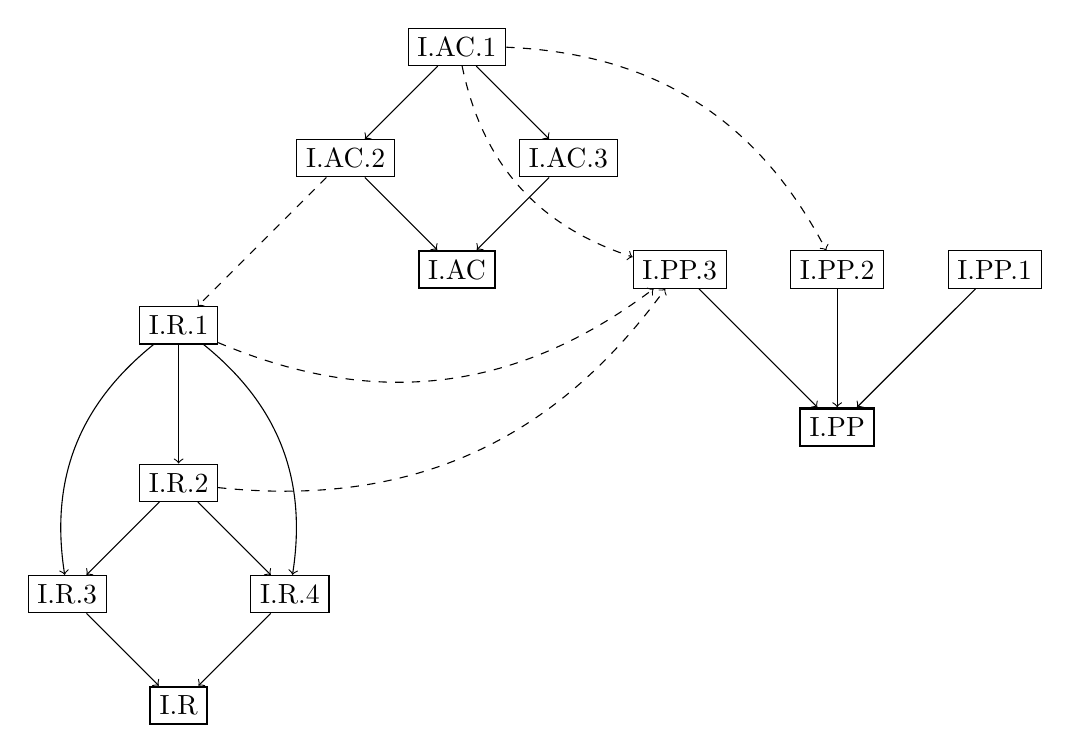
\begin{tikzpicture}[->, node distance=2cm]
		\node[draw=black] (iac1) {\code{I.AC.1}};
		\node[draw=black] (iac2) [below left of=iac1] {\code{I.AC.2}};
		\node[draw=black] (iac3) [below right of=iac1] {\code{I.AC.3}};
		\node[draw=black, thick] (iac) [below right of=iac2] {\code{I.AC}};

		\path (iac1) edge (iac2)
				(iac1) edge (iac3)
				(iac2) edge (iac)
				(iac3) edge (iac);
				
		\node[draw=black] (ir1) [below left of=iac2, node distance=3cm] {\code{I.R.1}};
		\node[draw=black] (ir2) [below of=ir1] {\code{I.R.2}};
		\node[draw=black] (ir3) [below left of=ir2] {\code{I.R.3}};
		\node[draw=black] (ir4) [below right of=ir2] {\code{I.R.4}};
		\node[draw=black, thick] (ir) [below right of=ir3] {\code{I.R}};
		
		\path (iac2) edge [dashed] (ir1);
		
		\path (ir1) edge (ir2)
				(ir1) edge [bend right] (ir3)
				(ir1) edge [bend left] (ir4)
				(ir2) edge (ir3)
				(ir2) edge (ir4)
				(ir3) edge (ir)
				(ir4) edge (ir);

		\node[draw=black] (ipp3) [below right of=iac3] {\code{I.PP.3}};
		\node[draw=black] (ipp2) [right of=ipp3] {\code{I.PP.2}};
		\node[draw=black] (ipp1) [right of=ipp2] {\code{I.PP.1}};
		\node[draw=black, thick] (ipp) [below of=ipp2] {\code{I.PP}};
		
		\path (iac1) edge [dashed, bend left] (ipp2);
		\path (iac1) edge [dashed, bend right] (ipp3)
				(ir1) edge [dashed, bend right] (ipp3)
				(ir2) edge [dashed, bend right] (ipp3);
		
		\path (ipp1) edge (ipp)
				(ipp2) edge (ipp)
				(ipp3) edge (ipp);
	\end{tikzpicture}
	\label{fig:attivita_inception_grafo}
\end{figure*}


\clearpage

\subsection{Diagramma di Gantt}

Rappresentiamo la temporizzazione delle attivit\`a attraverso le fasi del progetto e teniamo traccia del loro stato di esecuzione con una serie di diagrammi di Gantt.
Il tempo di esecuzione richiesto da ciascuna attivit\`a non rispecchia perfettamente i tempi previsti: alcune attivit\`a, come ad esempio la creazione degli use case o del glossario, sono state protratte nel tempo per procedere di pari passo con attivit\`a da cui dipendono.

Il diagramma di Gantt relativo alla fase di inception \`e rappresentato in figura \ref{fig:gantt_inception}.

%\begin{figure*}[tbh]
%	\centering
%     \begin{ganttchart}[
%			title/.style={fill={color1!10}},
%			title label font=\color{color2},
%			title left shift=.1,
%			title right shift=-.1,
%			title top shift=.05,
%			hgrid,
%			bar label font = \scriptsize,
%			group label font = \scriptsize,
%			milestone label font = \scriptsize,
%			x unit=1cm,
%%			milestone height = 0.2,
%			today=2016-04,
%			today label = {},
%			today rule/.style = {draw={color1!60}},
%			progress label text = {\pgfmathprintnumber[precision=0, verbatim]{#1}\%},
%			inline,
%			milestone inline label node/.append style={left=1mm},
%			time slot format={isodate-yearmonth},
%			compress calendar,
%		]{2016-02}{2016-08}
%           \gantttitlecalendar{year, month} \\
%%           \ganttbar{Sviluppo proposta}{2015-11-01}{2015-12-01} \\
%           \ganttbar{Inception}{2016-02}{2016-04} \\
%           \ganttmilestone{Conclusione inception}{2016-04} \\
%           \ganttbar{Elaboration}{2016-05}{2016-06} \\
%           \ganttmilestone{Conclusione elaboration}{2016-06} \\
%           \ganttbar{Construction}{2016-07}{2016-08} \\
%           \ganttmilestone{Conclusione construction}{2016-08}
%      \end{ganttchart}
%\end{figure*}

\begin{figure*}
\centering
\hspace*{-0.8cm}
\begin{ganttchart}[
			title/.style={fill={color1!10}},
			title label font=\color{color2},
			title left shift=.1,
			title right shift=-.1,
			title top shift=.05,
			hgrid,
			vgrid,
			bar label font = \scriptsize,
			group label font = \scriptsize,
			milestone label font = \scriptsize,
			x unit=2.2mm,
			milestone height = 0.2,
%			today=2016-05-04,
			today label = {},
			today rule/.style = {draw={color1!60}},
			progress label text = {\pgfmathprintnumber[precision=0, verbatim]{#1}\%},
			inline,
			milestone inline label node/.append style={left=1mm},
			time slot format={isodate},
		]{2016-02-22}{2016-05-15}
	\gantttitlecalendar{year, month} \\
	\ganttgroup[progress=100]{Analisi del contesto}{2016-02-22}{2016-04-10} \\
	\ganttbar[progress=100]{Raccolta informazioni contesto}{2016-02-22}{2016-03-22} \\
	\ganttbar[progress=100]{Studio business cases}{2016-03-01}{2016-03-22} \\
	\ganttbar[progress=100]{Studio di fattibilit\`a}{2016-03-2}{2016-04-06} \\
	\ganttbar[progress=100]{Stesura documento analisi contesto}{2016-03-14}{2016-04-10} \\
	\ganttgroup[progress=100]{Raccolta requisiti}{2016-03-09}{2016-05-04} \\
	\ganttbar[progress=100]{Definizione requisiti}{2016-03-09}{2016-04-18} \\
	\ganttbar[progress=100]{Specifica requisiti}{2016-03-28}{2016-04-27} \\
	\ganttbar[progress=100]{Creazione glossario}{2016-03-16}{2016-04-18} \\
	\ganttbar[progress=100]{Definizione use-case principali}{2016-03-20}{2016-04-18} \\
	\ganttbar[progress=100]{Stesura documento requisiti}{2016-03-16}{2016-05-04} \\
	\ganttgroup[progress=100]{Pianificazione progetto}{2016-03-25}{2016-04-28} \\
	\ganttbar[progress=100]{Definizione milestone}{2016-03-25}{2016-04-10} \\
	\ganttbar[progress=100]{Analisi dei rischi}{2016-03-25}{2016-04-10} \\
	\ganttbar[progress=100]{Analisi dei costi}{2016-03-29}{2016-04-16} \\
	\ganttbar[progress=100]{Stesura piano di progetto}{2016-03-25}{2016-04-28} \\
	\ganttmilestone[progress=100]{Prima revisione capo progetto}{2016-04-12}
	\ganttmilestone[progress=100]{Seconda revisione capo progetto}{2016-05-10}
\end{ganttchart}
\caption{\label{fig:gantt_inception}Diagramma di Gantt della fase di Inception.}
\end{figure*}

\begin{figure*}
	\centering
	\hspace*{-0.8cm}
	\begin{ganttchart}[
		title/.style={fill={color1!10}},
		title label font=\color{color2},
		title left shift=.1,
		title right shift=-.1,
		title top shift=.05,
		hgrid,
		vgrid,
		bar label font = \scriptsize,
		group label font = \scriptsize,
		milestone label font = \scriptsize,
		x unit=5mm,
		milestone height = 0.2,
		today=2016-09-06,
		today label = {},
		today rule/.style = {draw={color1!60}},
		progress label text = {\pgfmathprintnumber[precision=0, verbatim]{#1}\%},
		inline,
		milestone inline label node/.append style={left=1mm},
		time slot format={isodate},
		]{2016-09-01}{2016-09-20}
		\gantttitlecalendar{year, month} \\
		\ganttgroup[progress=75]{Specifica requisiti}{2016-09-01}{2016-09-10} \\
		\ganttbar[progress=75]{Specifica requisiti sistema}{2016-09-01}{2016-09-10} \\
		\ganttbar[progress=75]{Stesura documento requisiti}{2016-09-02}{2016-09-10} \\
		\ganttgroup[progress=30]{Definizione use case model}{2016-09-02}{2016-09-11} \\
		\ganttbar[progress=70]{Realizzazione diagrammi use case}{2016-09-03}{2016-09-11} \\
		\ganttbar[progress=35]{Specifica use case}{2016-09-03}{2016-09-11} \\
		\ganttbar[progress=30]{Stesura documento use case model}{2016-09-03}{2016-09-11} \\
		\ganttgroup[progress=0]{Definizione architettura sistema}{2016-09-03}{2016-09-12} \\
		\ganttbar[progress=0]{Definizione system boundary}{2016-09-03}{2016-09-12} \\
		\ganttbar[progress=0]{Stesura documento architettura sistema}{2016-09-05}{2016-09-12} \\
		\ganttmilestone[progress=0]{Terza revisione capo progetto}{2016-09-06}
	\end{ganttchart}
	\caption{\label{fig:gantt_elaboration}Diagramma di Gantt della fase di Elaboration.}
\end{figure*}


\clearpage

\section{Analisi dei costi}

La stima dei costi di realizzazione del progetto viene effettuata con la tecnica degli \emph{Use Case Points}.

Gli Use Case Points del progetto sono dati dalla somma di due addendi.

\paragraph{Unadjusted Use Case Weight}
	Misura il numero e la complessit\`a degli Use Case del sistema.

\paragraph{Unadjusted Actor Weight}
	Misura il numero e la complessit\`a degli attori del sistema.

Il valore ottenuto dalla somma di \code{UUCW} e \code{UAW} viene moltiplicato per due fattori.

\paragraph{Technical Complexity Factor}
	Misura la complessit\`a tecnica del sistema.

\paragraph{Environmental Complexity Factor}
	Misura la complessit\`a dell'ambiente in cui il sistema viene sviluppato.

\subsection{Unadjusted Use Case Weight}

Il \code{UUCW} assegna un punteggio a ciascun use case del sistema secondo la complessit\`a dello use case.

Il \code{UUCW} sar\`a determinato a individuazione degli use case ultimata.

\subsection{Unadjusted Actor Weight}

Il \code{UAW} sar\`a determinato a individuazione degli use case ultimata.

\subsection{Technical Complexity Factor}

Il \code{TCF} \`e un fattore moltiplicativo che tiene conto della complessit\`a tecnica del sistema in sviluppo.
Ciascun fattore tecnico ha un peso compreso fra $0.5$ e $2.0$.
A ciascun fattore tecnico viene assegnato un valore fra $0$ (fattore ininfluente) e $5$ (fattore essenziale)
Il \code{TCF} viene calcolato sommando il prodotto di peso e valore per ciascun fattore tecnico.

I valori assegnati sono indicati nella tabella seguente.
%I valori assegnati sono indicati nella tabella \ref{tab:tcf}.

\begin{center}
\begin{tabularx}{\columnwidth}{c X c c}
\toprule
\cellcolor{color2!10} Fatt. & \cellcolor{color2!10} Descrizione & \cellcolor{color2!10} Peso & \cellcolor{color2!10} Val. \\
\midrule
\code{T1} & Sistema distribuito & $2.0$ & 4 \\
\code{T2} & Obiettivi di performance/tempo di risposta & $1.0$ & 2 \\
\code{T3} & Efficienza lato utente & $1.0$ & 2 \\
\code{T4} & Complessit\`a processi interni & $1.0$ & 4 \\
\code{T5} & Riusabilit\`a del codice & $1.0$ & 3 \\
\code{T6} & Facilit\`a d'installazione & $0.5$ & 5 \\
\code{T7} & Facilit\`a d'utilizzo & $0.5$ & 4 \\
\code{T8} & Portabilit\`a inter-piattaforma & $2.0$ & 5 \\
\code{T9} & Manutenzione del sistema & $1.0$ & 5 \\
\code{T10} & Parallelismo/concorrenza & $1.0$ & 5 \\
\code{T11} & Sicurezza & $1.0$ & 5 \\
\code{T12} & Accesso terze parti & $1.0$ & 5 \\
\code{T13} & Addestramento utente & $1.0$ & 1 \\
\midrule
\multicolumn{3}{r}{Totale \code{TCF}} & 50 \\
\bottomrule
\end{tabularx}
%\caption{\label{tab:tcf} Fattori di complessit\`a tecnica.}
\end{center}

L'assegnamento dei valori \`e basato sulle seguenti considerazioni:
\begin{itemize}
	\item \code{T1}: il sistema sar\`a verosimilmente composto da pi\`u componenti distribuite, identificate dalle loro responsabilit\`a.
	\item \code{T2}: il sistema non ha particolari necessit\`a in termini di performance, le operazioni svolte non hanno particolare complessit\`a.
		Il tempo di risposta del sistema devono rientrare nei tempi di risposta di un generico sito web, dell'ordine dei pochi secondi, ed \`e quindi un fattore mediamente rilevante.
	\item \code{T3}: l'efficienza lato utente del sistema \`e un fattore poco rilevante rispetto a altri fattori come la sicurezza del sistema (\code{T11}).
	\item \code{T4}: i processi interni del sistema \`e presumibile siano molto complessi.
	\item \code{T5}: la riusabilit\`a del codice prodotto \`e un fattore rilevante del progetto.
		\`E indirettamente correlato alla manutebilit\`a del sistema, e direttamente correlato alla possibilit\`a di implementare \emph{plugin} per il sistema.
	\item \code{T6}: la facilit\`a d'installazione \`e un fattore essenziale.
		Il software \`e destinato a enti bancari, e l'installazione sar\`a curata da membri della nostra societ\`a come parte preponderante della fase di Transition.
	\item \code{T7}: la facilit\`a d'utilizzo \`e una componente molto importante del sistema.
		Il sistema in sviluppo riguarda questioni finanziarie della vita del singolo, per le quali la facilit\`a d'uso non \`e importante quanto altre questioni, principalmente la sicurezza del sistema e dei risparmi degli utenti: a titolo d'esempio, se operazioni sensibili come inviare un bonifico richiedono pi\`u step da completare con attenzione \`e ragionevole pensare che sia pi\`u difficile effettuare un bonifico per errore.
		La facilit\`a d'uso \`e pi\`u rilevante per i dipendenti della banca.
	\item \code{T8}: la portabilit\`a del software sviluppato fra pi\`u piattaforme \`e un fattore essenziale del progetto, poich\'e non si possono avere informazioni precise in anticipo sulle macchine utilizzate da chi acquister\`a il nostro software.
	\item \code{T9}: la manutenzione del sistema \`e una delle parti fondamentali della fase di transition, ed \`e quindi un fattore essenziale nello sviluppo dello stesso.
	\item \code{T10}: le operazioni che dovr\`a svolgere il sistema di home banking in sviluppo avranno sicuramente degli aspetti di gestione della concorrenza, ad esempio nella gestione delle operazioni di un utente.
	\item \code{T11}: la sicurezza \`e uno degli aspetti fondamentali del progetto in quanto requisito non funzionale.
	\item \code{T12}: l'accesso a parti terze \`e uno degli aspetti fondamentali del progetto in quanto requisito di dominio.
	\item \code{T13}: l'addestramento utente \`e praticamente irrilevante.
		Gli utenti finali del sistema di Home Banking (clienti della banca) non possono essere addestrati.
		I dipendenti della banca possono essere addestrati, ma la necessit\`a di addestramento dovrebbe essere mitigata dalla facilit\`a d'uso del software (fattore \code{T7}).
\end{itemize}

\subsection{Environmental Complexity Factor}

Il \code{ECF} \`e un fattore moltiplicativo che tiene conto della complessit\`a dell'ambiente in cui il software viene sviluppato.
Ciascun fattore ambientale ha un peso compreso fra $0.5$ e $2.0$.
A ciascun fattore ambientale viene assegnato un valore fra $0$ (fattore ininfluente) e $5$ (fattore essenziale)
Il \code{ECF} viene calcolato sommando il prodotto di peso e valore per ciascun fattore ambientale.

I valori assegnati sono indicati nella tabella seguente.
%I valori assegnati sono indicati nella tabella \ref{tab:ecf}.

\begin{center}
\begin{tabularx}{\columnwidth}{c X r r}
\toprule
\cellcolor{color2!10} Fatt. & \cellcolor{color2!10} Descrizione & \cellcolor{color2!10} Peso & \cellcolor{color2!10} Val. \\
\midrule
\code{E1} & Familiarit\`a con processo software adottato & $1.5$ & 4 \\
\code{E2} & Esperienza nel dominio dell'applicazione & $0.5$ & 4 \\
\code{E3} & Esperienza del team con orientazione a oggetti & $1.0$ & 5 \\
\code{E4} & Capacit\`a primo analista & $0.5$ & 4 \\
\code{E5} & Motivazione del team & $1.0$ & 4 \\
\code{E6} & Stabilit\`a dei requisiti & $2.0$ & 4 \\
\code{E7} & Staff part-time & $-1.0$ & 0 \\
\code{E8} & Linguaggio di programmazione ostico & $-1.0$ & 3 \\
\midrule
\multicolumn{3}{r}{Totale \code{ECF}} & 28 \\
\bottomrule
\end{tabularx}
%\caption{\label{tab:ecf} Fattori di complessit\`a ambientale.}
\end{center}

L'assegnamento dei valori \`e basato sul fatto che il software in sviluppo \`e \emph{sensibile}, in quanto concerne transazioni economiche di privati e presenta quindi problematiche importanti legate a sicurezza, aspetti legali, e privacy degli utenti.
Il progetto richiede quindi un team competente ed esperto tanto nel dominio quanto in aspetti legati al processo adottato e in generale alle pratiche di sviluppo \emph{object oriented}.
Per queste stesse considerazioni, e per i tempi di sviluppo condizionati dall'evoluzione dello scenario legale (relativo al dominio bancario) italiano, la stabilit\`a dei requisiti \`e un fattore molto rilevante.

\subsection{Use Case Points e previsione di costo}

Gli Use Case Points saranno determinati a individuazione degli use case ultimata.


\clearpage

\section{Rapporto fra rischi e progetto}

La realizzazione di un sistema sensibile qual \`e un sistema di Home Banking \`e inerentemente \emph{rischiosa}.

Errori in fase di raccolta dei requisiti e analisi possono portare a un sistema sottodimensionato o non conforme alle necessit\`a del nostro target di clienti (un insieme eterogeneo di istituti bancari).

Errori in fase di progettazione e di sviluppo possono compromettere l'usabilit\`a del sistema da parte degli utenti (i clienti della banca) risultando in un danno di immagine e in una perdita di fiducia nel \emph{brand} che utilizza il nostro sistema.

Errori gravi in fase di progettazione e di sviluppo possono compromettere la sicurezza del sistema, con possibili perdite monetarie per banche e clienti di queste, e responsabilit\`a penali per il nostro gruppo.

Errori in fase di \emph{deployment}, similmente, possono compromettere usabilit\`a e sicurezza del sistema.

In questo scenario la valutazione dei rischi deve essere portata avanti per tutta la durata del progetto e integrata nel \emph{workflow} di sviluppo, influenzando le scelte fatte in ogni passo, e aggiornando la valutazione dei rischi in seguito a ogni scelta.

\subsection{Classificazione dei rischi}

I rischi identificati sono raggruppati nel seguito per fase di processo.
Rischi differenti possono emergere in seguito a, o venire mitigati da, particolari scelte, o non essere rilevanti in una specifica fase del processo di sviluppo.

Definiamo un rischio come un evento che pu\`o verificarsi durante il processo.
A ogni rischio associamo:
\begin{itemize}
	\item una stima della probabilit\`a con cui l'evento pu\`o verificarsi;
	\item una stima dell'impatto che l'evento avrebbe sul processo.
\end{itemize}
Distinguiamo 5 classi di rischio basate sulla stima di probabilit\`a e 4 classi basate sulla stima dell'impatto.

Le classi di probabilit\`a sono:
\begin{itemize}
	\item ``probabilit\`a massima/certa'' (\code{CP}) se la probabilit\`a che l'evento si verifichi \`e stimata superiore all'80\%;
	\item ``probabilit\`a alta'' (\code{HP}) se la probabilit\`a che l'evento si verifichi \`e stimata fra il 60\% e l'80\%;
	\item ``probabilit\`a media'' (\code{MP}) se la probabilit\`a che l'evento si verifichi \`e stimata fra il 40\% e l'60\%;
	\item ``probabilit\`a bassa'' (\code{LP}) se la probabilit\`a che l'evento si verifichi \`e stimata fra il 20\% e l'40\%;
	\item ``probabilit\`a minima/nulla'' (\code{NP}) se la probabilit\`a che l'evento si verifichi \`e stimata inferiore al 20\%.
\end{itemize}

Le classi di impatto sono stabilite in base alla quantit\`a di iterazioni e/o fasi del progetto che dovranno essere eseguite per evitare il fallimento del progetto, e in base al danno economico che il verificarsi dell'evento comporterebbe.
Le classi di impatto sono:
\begin{itemize}
	\item ``impatto massimo'' (\code{ED}) se \`e necessario ritornare alla fase di Inception, scartando ogni progresso fatto, o se di fatto il progetto \`e fallito;
	\item ``impatto alto'' (\code{HD}) se \`e necessario tornare alla fase precedente, o se le possibilit\`a di profitto del progetto sono seriamente ridotte;
	\item ``impatto medio'' (\code{MD}) se \`e necessario ripetere un'iterazione all'interno della fase attuale, o se le probabilit\`a di profitto del progetto sono ridotte;
	\item ``impatto basso'' (\code{LD}) se \`e possibile proseguire il processo senza ripetere fasi o iterazioni, o se le possibilit\`a di profitto del progetto sono sostanzialmente immutate.
\end{itemize}

\begin{figure}
	\resizebox{\columnwidth}{!}{
	\begin{tikzpicture}
		\begin{axis}[
			scale only axis,
			width=\columnwidth,
			xmin=-0.1, ymin=-0.5,
			ymax=4,
			ticks=none,
			domain=0:2,
			xlabel={Perdita su guadagno atteso},
			ylabel={Tempo rielaborazione progetto},
			axis lines=left,
			samples=200
        ]
		    \path[name path=axis] (axis cs:0,0) -- (axis cs:1,0);
			\addplot[name path=l, shift={(-36, -12)},thick,green] {1/x};
			\addplot[name path=m, shift={(-18, -6)},thick,yellow] {1/x};
   			\addplot[name path=h, thick,red] {1/x};
   			\node [] at (axis cs:0.2,0) {basso};
   			\node [] at (axis cs:0.6,0.3) {medio};
   			\node [] at (axis cs:1.0,0.6) {alto};
   			\node [] at (axis cs:1.4,1.2) {massimo};

		\end{axis}
	\end{tikzpicture}
	}
	\caption{Classificazione impatto dei rischi rispetto a tempo lavoro richiesto e impatto sul guadagno finale.}
	\label{fig:rappresentazione_impatto}
\end{figure}

\subsection{Identificazione dei rischi}

Identifichiamo i rischi con la codifica ottenuta concatenando i seguenti elementi, usando un \emph{underscore} come separatore:
\begin{itemize}
	\item il prefisso comune \code{RIS}
	\item una sequenza di 4-6 lettere (identificativo mnemonico)
	\item un identificativo di probabilit\`a (in ordine decrescente \code{CP}, \code{HP}, \code{MP}, \code{LP}, \code{NP})
	\item un identificativo dell'impatto (in ordine decrescente \code{ED}, \code{HD}, \code{MD}, \code{LD})
	\item un intero strettamente positivo (unico per ogni rischio).
\end{itemize}
In contesti in cui \`e necessario essere concisi \`e possibile identificare i rischi utilizzando unicamente il prefisso \code{RIS} e l'intero assegnato al rischio.

Ad esempio, il rischio ``ritardo nella consegna del progetto'', con probabilit\`a alta e impatto basso, potrebbe essere identificato dalla stringa \code{RIS\_DELAY\_HP\_LD\_1}, o per brevit\`a come \code{RIS\_1}.

Seguendo un approccio \emph{RMMM} individuiamo dei piani di \emph{\cellcolor{color2!10}Mitigation} (per ridurre la probabilit\`a dell'evento), \emph{\cellcolor{color2!10}Monitoring} (per controllare il verificarsi dell'evento) e \emph{\cellcolor{color2!10}Management} (per ridurre le perdite a evento avvenuto).
Il piano di \emph{Monitoring} di un rischio rappresenta un \emph{trigger} per la gestione (\emph{Management}) del rischio stesso.

\section{Rischi individuati durante l'Inception}

\subsection{\code{RIS\_1} - Ritardo nella \emph{delivery} del progetto}

\begin{ptable}{3}
\ptitlerow{\bf Ritardo nella \emph{delivery} del progetto}
\pcells{ID & Probabilit\`a & Impatto}
\pcells{$\code{RIS\_DELAY\_MP\_HD\_1}$ & 50\% & alto}
\pline
\ptitlerow{Descrizione}
\prow{
Il progetto si colloca in un ambiente con \emph{internet time}, e in particolare in una situazione verosimilmente \emph{first comer takes all}: presentare un prodotto in un mercato ancora vuoto porter\`a a guadagni molto pi\`u elevati rispetto al presentarlo in un mercato non vuoto.
}
\pline
\ptitlerow{Mitigation}
\prow{
Stabilire piano di progetto accurato e insieme di requisiti gestibile per consegnare un prodotto competitivo in tempi brevi.
Utilizzare approccio iterativo nell'implementazione per produrre iterazioni successive di software via via pi\`u complete ma tutte singolarmente vendibili.
Monitorare costantemente fattibilit\`a del progetto, e individuare \emph{bottleneck} di sviluppo in anticipo, ove possibile.
}
\pline
\ptitlerow{Monitoring}
\prow{
Controllare periodicamente stato sviluppo di aziende concorrenti, se presenti.
Avviare operazioni di \emph{management} qualora un prodotto concorrente venga rilasciato sul mercato.
}
\pline
\ptitlerow{Management}
\prow{
Rilasciare prodotto dell'ultima iterazione di sviluppo.
}
\end{ptable}

\subsection{\code{RIS\_2} - Funzionalit\`a non sufficienti per clienti}

\begin{ptable}{3}
\ptitlerow{\bf Funzionalit\`a non sufficienti per clienti}
\pcells{ID & Probabilit\`a & Impatto}
\pcells{$\code{RIS\_REQINS\_MP\_ED\_2}$ & 50\% & massimo}
\pline
\ptitlerow{Descrizione}
\prow{
Il progetto ha come target un insieme eterogeneo di enti bancari, con necessit\`a eterogenee dal punto di vista dell'Home Banking.
Se le funzionalit\`a del software prodotto non soddisferanno le necessit\`a di un numero sufficiente di enti bancari il software non avr\`a mercato, con ovvie e pesanti perdite economiche.
}
\pline
\ptitlerow{Mitigation}
\prow{
Lavorare costantemente sui requisiti, mantenendoli flessibili.
Interagire attivamente con possibili clienti per mantenere visione realistica dei requisiti effettivi.
}
\pline
\ptitlerow{Monitoring}
\prow{
Colloqui periodici con personale di enti bancari per assicurare non divergenza fra requisiti raccolti e necessit\`a dei clienti.
Avviare operazioni di \emph{management} non appena venga individuata una divergenza fra i requisiti reali e i requisiti raccolti.
}
\pline
\ptitlerow{Management}
\prow{
Reiterare fasi di sviluppo per implementare nuovi requisiti.
}
\end{ptable}

\subsection{\code{RIS\_3} - Problematiche con strumenti software}

\begin{ptable}{3}
\ptitlerow{\bf Problematiche con strumenti software}
\pcells{ID & Probabilit\`a & Impatto}
\pcells{$\code{RIS\_PRSOFT\_LP\_LD\_3}$ & 30\% & basso}
\pline
\ptitlerow{Descrizione}
\prow{
Il software prodotto dovr\`a utilizzare diversi componenti di terze parti per accelerare lo sviluppo e aumentare le garanzie di sicurezza.
Problematiche di questi strumenti software (ad es. bug, falle di sicurezza) potrebbero inficiare lo sviluppo del progetto.
}
\pline
\ptitlerow{Mitigation}
\prow{
Utilizzare strumenti software di comprovata affidabilit\`a.
In caso di software proprietario, stabilire accordi commerciali che tutelino dalla presenza di problemi software e che garantiscano un tempo di recupero massimo da problematiche software.
}
\pline
\ptitlerow{Monitoring}
\prow{
Mantenere contatti regolari con produttori del software utilizzato e seguire fonti di informazione specializzate dell'ambiente, controllando presenza di problematiche con gli strumenti software.
Avviare operazioni di \emph{management} non appena emergono notizie di problematiche con uno o pi\`u dei software utilizzati.
}
\pline
\ptitlerow{Management}
\prow{
In caso di problematiche con software proprietario, attenderne soluzione e applicare aggiornamenti non appena disponibili.
In caso di problematiche con software open-source, contribuire alla risoluzione del problema qualora gli sviluppatori abbiano la competenza necessaria e sia possibile dedicare risorse al compito.
In presenza di software alternativo che possa rimpiazzare il software problematico, qualora sia possibile effettuare \emph{refactoring} a un costo di tempo o monetario contenuto, sostituire il software problematico con l'alternativa disponibile.
}
\end{ptable}

\subsection{\code{RIS\_4} - Complessit\`a progetto sottovalutata}

\begin{ptable}{3}
\ptitlerow{\bf Complessit\`a progetto sottovalutata}
\pcells{ID & Probabilit\`a & Impatto}
\pcells{$\code{RIS\_COMPLX\_LP\_HD\_4}$ & 20\% & alto}
\pline
\ptitlerow{Descrizione}
\prow{
Sottostimare la complessit\`a del software da realizzare pu\`o essere causa di rallentamenti nello sviluppo, errori nell'analisi dei requisiti o di un prodotto finale non performante.
}
\pline
\ptitlerow{Mitigation}
\prow{
Aumentare ragionevolmente stime in caso di incertezza.
Prestare particolare attenzione alle fasi iniziali di analisi.
}
\pline
\ptitlerow{Monitoring}
\prow{
Realizzare prototipi a partire dalla fase di analisi per avere una misura reale della fattibilit\`a e complessit\`a del sistema.
Controllare complessit\`a dei prototipi e il rapporto di questa con la complessit\`a del sistema.
Avviare operazioni di \emph{management} nel momento in cui viene verificata la presenza di fonti di complessit\`a non previste.
}
\pline
\ptitlerow{Management}
\prow{
Individuare la fonte dell'aumento di complessit\`a e se possibile modificare requisiti, architettura o design del sistema per ridurre la complessit\`a.
Rieseguire le stime.
Ripetere le iterazioni necessarie a implementare le modifiche o tornare a una fase precedente qualora non fosse evitabile.
}
\end{ptable}

\subsection{\code{RIS\_5} - Normative legali violate}

\begin{ptable}{3}
\ptitlerow{\bf Normative legali violate}
\pcells{ID & Probabilit\`a & Impatto}
\pcells{$\code{RIS\_LEGAL\_MP\_HD\_5}$ & 40\% & massimo}
\pline
\ptitlerow{Descrizione}
\prow{
Il software di Home Banking prodotto deve rispettare le normative vigenti, tanto dal lato utenti della banca quanto dal lato ente bancario.
Violare le normative avrebbe conseguenze penali per gli sviluppatori del software.
}
\pline
\ptitlerow{Mitigation}
\prow{
Mantenere contatti con esperti del settore per conoscere quali normative vadano rispettate.
}
\pline
\ptitlerow{Monitoring}
\prow{
Mantenere contatti con esperti del settore per verificare legalit\`a del software prodotto.
Avviare operazioni di \emph{management} nel momento in cui uno o pi\`u esperti del settore indicano la presenza di normative legali violate.
}
\pline
\ptitlerow{Management}
\prow{
Implementare soluzioni per rimuovere le violazioni delle normative.
}
\end{ptable}

\subsection{\code{RIS\_6} - Violazione sicurezza durante sviluppo}

\begin{ptable}{3}
\ptitlerow{\bf Violazione sicurezza durante sviluppo}
\pcells{ID & Probabilit\`a & Impatto}
\pcells{$\code{RIS\_DEVSEC\_LP\_HD\_6}$ & 20\% & alto}
\pline
\ptitlerow{Descrizione}
\prow{
I computer e i server su cui il software verr\`a sviluppato potrebbero essere bersaglio di attacchi informatici volti a ottenere informazioni di sicurezza e/o a inserire vulnerabilit\`a nel software.
}
\pline
\ptitlerow{Mitigation}
\prow{
Investire risorse per individuare e prevenire falle di sicurezza nei computer e nel Version Control System utilizzati in fase di sviluppo.
Effettuare regolarmente back-up del codice sorgente su supporti \emph{off the grid}.
}
\pline
\ptitlerow{Monitoring}
\prow{
A sviluppo iniziato investire risorse per tenere sotto controllo accessi ai computer e al Version Control System, e l'integrit\`a dei file ivi presenti.
Avviare operazioni di \emph{management} nel momento in cui viene riscontrata una violazione del sistema.
}
\pline
\ptitlerow{Management}
\prow{
In caso di software infettato effettuare un \emph{roll-back} tramite il Version Control System utilizzato all'ultima versione non compromessa, effettuare controlli su software rilasciato e rimuovere software infetto dalla circolazione.

In caso di \emph{leakage} di informazioni riservate sostituibili (chiavi private, certificati, etc) effettuare la sostituzione ove possibile.
}
\end{ptable}

\subsection{\code{RIS\_7} - Software presenta falle di sicurezza}

\begin{ptable}{3}
\ptitlerow{\bf Software presenta falle di sicurezza}
\pcells{ID & Probabilit\`a & Impatto}
\pcells{$\code{RIS\_SECUR\_MP\_ED\_7}$ & 50\% & massimo}
\pline
\ptitlerow{Descrizione}
\prow{
Sviluppare software sicuro \emph{ex-novo} \`e notoriamente difficile e facilmente soggetto ad errori.
Particolare attenzione deve essere dedicata affinch\'e il software prodotto non contenga falle di sicurezza.
}
\pline
\ptitlerow{Mitigation}
\prow{
Adottare pratiche di sviluppo difensivo.
Riutilizzare moduli e componenti software di comprovata affidabilit\`a e gi\`a soggetti a test esaustivi per massimizzare la stratificazione e disaccoppiare la struttura del software.
}
\pline
\ptitlerow{Monitoring}
\prow{
Investire risorse per cercare vulnerabilit\`a nel software durante lo sviluppo.
Avviare operazioni di \emph{management} qualora venga riscontrata la presenza di vulnerabilit\`a nel software prodotto.
}
\pline
\ptitlerow{Management}
\prow{
Risolvere la vulnerabilit\`a, aggiornare software gi\`a \emph{deployed}.
}
\end{ptable}

\subsection{\code{RIS\_8} - Problematiche sistema di bidding}

\begin{ptable}{3}
\ptitlerow{\bf Problematiche sistema di bidding}
\pcells{ID & Probabilit\`a & Impatto}
\pcells{$\code{RIS\_BIDPR\_MP\_MD\_8}$ & 40\% & medio}
\pline
\ptitlerow{Descrizione}
\prow{
La funzionalit\`a di bidding presente nei requisiti \`e una funzionalit\`a nuova e non presente in altri contesti.
Nella fase di definizione dei requisiti \`e emerso il rischio di una complessit\`a troppo elevata del sistema per gli utenti di HBS (sia per i clienti che per i manager della banca).
Un sistema di bidding troppo complesso per i clienti della banca potrebbe non venire utilizzato, e trasformarsi quindi in una funzionalit\`a inutile.
Un sistema di bidding troppo complesso per i manager della banca potrebbe portare i manager a impostare non correttamente i parametri di accettazione automatica dei \emph{bid} e risultare in perdite per l'istituto bancario.
}
\pline
\ptitlerow{Mitigation}
\prow{
Effettuare diverse e ripetute fasi di testing del sistema durante lo sviluppo del sistema con manager di enti bancari interessati a adottare HBS e con persone di varia provenienza sociale e con livello di alfabetizzazione digitale diversificato.
}
\pline
\ptitlerow{Monitoring}
\prow{
Registrare opinioni e pareri dei soggetti delle fasi di testing, registrare facilit\`a di traduzione dell'intenzione in azione con il sistema di bidding sviluppato.
Avviare fase di \emph{management} qualora la maggioranza dei soggetti delle fasi di testing abbia problemi a utilizzare il sistema di bidding.
}
\pline
\ptitlerow{Management}
\prow{
Reiterare analisi e sviluppo del sistema di bidding utilizzando i dati raccolti nelle fasi di testing per effettuare un \emph{refactoring} delle sezioni problematiche del software.
}
\end{ptable}

\section{Evoluzione dei rischi}

Durante lo sviluppo terremo traccia dell'evoluzione dei rischi, monitorando in particolare come cambia la probabilit\`a di un rischio e il suo impatto sul progetto.


\clearpage

\section{Registro modifiche}

\subsection{Inception}

\subsubsection{I iterazione}

Prima stesura documento.

\subsubsection{II iterazione}

Aggiunte revisioni \code{REV\_01\_01}, \code{REV\_01\_02}, \code{REV\_01\_03}, \code{REV\_01\_04}.
Terminata definizione dei milestone.
Aggiunti \emph{trigger} a rischi.
Individuati i fattori di complessit\`a tecnologici e ambientali.
Aggiunto rischio \code{RIS\_8} (problematiche sistema di bidding) individuato nella definizione dei requisiti.

\subsubsection{III iterazione}

Documento inalterato.

\subsection{Elaboration}

\subsubsection{I iterazione}

Aggiunto diagramma di Gantt per fase di Elaboration.

\subsubsection{II iterazione}

Aggiornati UCP.
Aggiornato diagramma di Gantt.
Integrato diagramma di Gantt fase di Construction in diagramma di Gantt fase di Elaboration.
Aggiornata analisi dei costi.

\subsection{Construction}

\subsubsection{I iterazione}

Aggiornato diagramma di Gantt.
Aggiornate deadline milestone.

\subsubsection{II iterazione}

Documento inalterato.

\end{document}
